\documentclass[a4paper]{llncs}
\usepackage{amsmath}

\usepackage{tikz}
\usetikzlibrary{positioning}
\usetikzlibrary{calc}
\usetikzlibrary{arrows,shapes,backgrounds}

\newcommand{\vphi}{\vec{\varphi}}
\newcommand{\vi}{{\vec{i}}}
\newcommand{\vj}{{\vec{j}}}
\newcommand{\vmu}{\vec{\mu}}

\title{ GPU-accelerated and CPU SIMD Optimized \\ Monte Carlo Simulation of $\phi^4$ Model}
\author{Piotr Bialas\inst{1} \and Jakub Kowal\inst{1} \and Adam Strzelecki\inst{1}}
\institute{Faculty of Physics, Astronomy and Applied Computer Science\\
Jagiellonian University\\
ul. Reymonta 4, 30-059 Krakow, Poland }
\begin{document}


\maketitle


\section{The model}
This contribution is concerned with an efficient implementation of the
Monte-Carlo simulations of the $\varphi^4$ model\cite{parisi}. The problem is
defined as follows: having a vector field $\vphi$ defined on a regular
rectangular two or three dimensional grid we want to generate the
field configurations with probability proportional to
\begin{equation}
e^{-H(\vphi)}
\end{equation}
where 
\begin{equation}\label{eq:ham}\begin{split} 
H(\varphi)&=\sum_{\vi}\Biggl(
\frac{1}{2}\sum_{\mu=1}^d(\vphi_{\vi+\hat{\mu}}-\vphi_{\vi})^2
+\frac{\mu^2}{2}|\vphi_{\vi}|^2+
\frac{g}{24}(|\vphi_{\vi}|^2)^2\\
&\phantom{=\sum_{\vi}\bigl(}+
\frac{1}{2\Lambda}\Bigl(\sum_{\mu=1}^d(\vphi_{\vi+\hat{\mu}}-2\vphi_{\vi}+\vphi_{\vi-\vmu})\Bigr)^2\Biggr).
\end{split}
\end{equation}
In the above expression $\vi$ denotes the grid point,
$\vphi_\vi$ denotes the $N$ component vector at the grid point $\vi$
 and $\vmu$ denotes the unit displacement on the grid in direction $\mu$. 

The actual  generation is done by the mean of the Metropolis  algorithm as follows: for a given lattice point $\vj$ we produce a new field 
\begin{equation}
\widetilde{\vphi}_\vj=\vphi_\vj+\vec{\epsilon}
\end{equation}
where $\epsilon$ is some random vector. The we calculate the difference 
$\Delta H = H(\widetilde{\vphi})-H(\vphi)$.
We then replace $\vphi_\vj$ with $\widetilde{\vphi}_\vj$ with the probability
\begin{equation}
P=\max\left\{1,\exp(-\Delta H)\right\}.
\end{equation}
The crucial feature of this algorithm is that the $\Delta H$ depends
only on the immediate neighbourhood of the point $\vj$. In our case
because of the lats term in \eqref{eq:ham} this neigborhood is
extended compared to usual nearest neigbours (see figure~\ref{fig:nn}). 

\begin{figure}
\begin{center} 
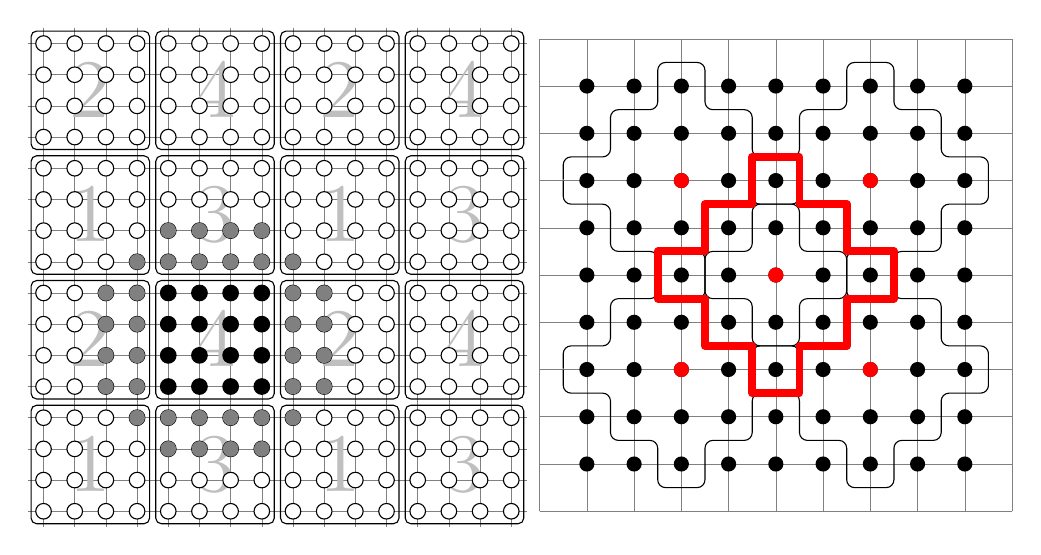
\begin{tikzpicture}[scale=0.6]
\begin{scope}[scale=0.66]
\draw[very thin, gray] (-0.5,-0.5) grid (15.5,15.5);

\foreach \x in {0,8}
\foreach \y in {0,8} 
\draw[xshift=\x cm, yshift = \y cm]
node[lightgray,scale=3] at (1.5cm,1.5) {$1$} 
node[lightgray,scale=3] at (1.5cm,5.5) {$2$} 
node[lightgray,scale=3] at (5.5cm,1.5) {$3$} 
node[lightgray,scale=3] at (5.5cm,5.5) {$4$} ;

\foreach \x in {0,...,15} 
 \foreach \y in {0,...,15} 
{
  \fill[white] (\x, \y) circle(0.25);
  \draw[black] (\x, \y) circle(0.25);
}

%\draw[xshift=-0.5cm,yshift=-0.5cm,step=4cm] (0cm,0cm) grid (16cm,16cm); 

\foreach \x in {4,...,7} 
\foreach \y in {4,...,7} 
{
  \fill[black] (\x, \y) circle(0.25);

}

\foreach \x in {4,...,7} 
\foreach \y in {2,3,8,9} 
{
  \fill[gray] (\x, \y) circle(0.25);

}

\foreach \x in {2,3,8,9} 
\foreach \y in {4,...,7} 
{
  \fill[gray] (\x, \y) circle(0.25);

}

\foreach \p in {(3,3),(3,8),(8,3),(8,8) }
  \fill[gray] \p circle(0.25);

\foreach \x in {0,4,...,12} 
\foreach \y in {0,4,...,12}
{
  \draw[black,xshift=\x cm, yshift=\y cm, rounded corners = 2pt] (-.4,-0.4) rectangle (3.4cm,3.4cm);
}

\end{scope}
\begin{scope}[xshift=13.5cm,yshift=3cm]
%\draw[->,rounded corners=0.2cm,shorten >=2pt] (0,2)-- (1,2);
%\draw (0,0) grid (4,4);
\draw[help lines] (-3.0,-3.0) grid (7.0,7.0);    

%punkty
%\foreach \c in {(0,0),(0,1),(1,0),(4,4),(4,3),(3,4),(0,4),(0,3),(3,0),(4,0),(1,4),(4,1),(2,1),(1,2),(3,2),(2,3),(1,1),(1,3),(3,1),(3,3),(0,2),(4,2),(2,0),(2,4)}
%    \fill \c + (0.0,0.0) circle (0.16);

%punkty
\foreach \x in {-2,-1,0,1,2,3,4,5,6}{
      \foreach \y in {-2,-1,0,1,2,3,4,5,6}{ 
		\fill (\x,\y) + (0.0,0.0) circle (0.16);
	}
}

%punkty dla ktorego dokonujemy aktualizacji    


%zasieg sasiedztwa g³ownego 
\draw[rounded corners=0.1cm,shorten >=2pt]
	(-0.5,2.0)-- ++(-0,-0.5)-- ++(1,0)-- ++(-0,-0.5)-- ++(-0,-0.5)-- ++(1,0)-- ++(-0,-1.0)-- ++(1,0)
	-- ++(-0,1.0)-- ++(1,0)-- ++(-0,1.0)-- ++(1,0)-- ++(0,1)-- ++(-1,0)-- ++(0,1)-- ++(-1,0)-- ++(0,1)
	-- ++(-1,0)-- ++(0,-1)-- ++(-1,0)-- ++(0,-1)--  ++(-1,0)-- ++(0,-0.6); 

%zasieg sasiedztwa NW
\draw[rounded corners=0.1cm,shorten >=2pt]
	(-2.5,4.0)-- ++(-0,-0.5)-- ++(1,0)-- ++(-0,-0.5)-- ++(-0,-0.5)-- ++(1,0)-- ++(-0,-1.0)-- ++(1,0)
	-- ++(-0,1.0)-- ++(1,0)-- ++(-0,1.0)-- ++(1,0)-- ++(0,1)-- ++(-1,0)-- ++(0,1)-- ++(-1,0)-- ++(0,1)
	-- ++(-1,0)-- ++(0,-1)-- ++(-1,0)-- ++(0,-1)--  ++(-1,0)-- ++(0,-0.6); 

%zasieg sasiedztwa g³ownego SW
\draw[rounded corners=0.1cm,shorten >=2pt]
	(-2.5,-0.0)-- ++(-0,-0.5)-- ++(1,0)-- ++(-0,-0.5)-- ++(-0,-0.5)-- ++(1,0)-- ++(-0,-1.0)-- ++(1,0)
	-- ++(-0,1.0)-- ++(1,0)-- ++(-0,1.0)-- ++(1,0)-- ++(0,1)-- ++(-1,0)-- ++(0,1)-- ++(-1,0)-- ++(0,1)
	-- ++(-1,0)-- ++(0,-1)-- ++(-1,0)-- ++(0,-1)--  ++(-1,0)-- ++(0,-0.6); 
	
%zasieg sasiedztwa g³ownego NE
\draw[rounded corners=0.1cm,shorten >=2pt]
	(1.5,4.0)-- ++(-0,-0.5)-- ++(1,0)-- ++(-0,-0.5)-- ++(-0,-0.5)-- ++(1,0)-- ++(-0,-1.0)-- ++(1,0)
	-- ++(-0,1.0)-- ++(1,0)-- ++(-0,1.0)-- ++(1,0)-- ++(0,1)-- ++(-1,0)-- ++(0,1)-- ++(-1,0)-- ++(0,1)
	-- ++(-1,0)-- ++(0,-1)-- ++(-1,0)-- ++(0,-1)--  ++(-1,0)-- ++(0,-0.6); 
	
%zasieg sasiedztwa g³ownego SE
\draw[rounded corners=0.1cm,shorten >=2pt]
	(1.5,-0.0)-- ++(-0,-0.5)-- ++(1,0)-- ++(-0,-0.5)-- ++(-0,-0.5)-- ++(1,0)-- ++(-0,-1.0)-- ++(1,0)
	-- ++(-0,1.0)-- ++(1,0)-- ++(-0,1.0)-- ++(1,0)-- ++(0,1)-- ++(-1,0)-- ++(0,1)-- ++(-1,0)-- ++(0,1)
	-- ++(-1,0)-- ++(0,-1)-- ++(-1,0)-- ++(0,-1)--  ++(-1,0)-- ++(0,-0.6); 
	
%oznaczenie glownej sieci
 \draw[line width=0.1cm,color=red,cap=round,join=round] (-0.5,2.0)-- ++(-0,-0.5)-- ++(1,0)-- ++(-0,-0.5)-- ++(-0,-0.5)-- ++(1,0)-- ++(-0,-1.0)-- ++(1,0)
	-- ++(-0,1.0)-- ++(1,0)-- ++(-0,1.0)-- ++(1,0)-- ++(0,1)-- ++(-1,0)-- ++(0,1)-- ++(-1,0)-- ++(0,1)
	-- ++(-1,0)-- ++(0,-1)-- ++(-1,0)-- ++(0,-1)--  ++(-1,0)-- ++(0,-0.6); 

\fill[red] (2,2) circle(0.16);
\fill[red] (0,4) circle(0.16);  
\fill[red] (-0,-0) circle(0.16);  
\fill[red] (4,0) circle(0.16);  
\fill[red] (4,4) circle(0.16);      
 
   \end{scope} 
%end
\end{tikzpicture}
\end{center}
\caption{\label{fig:nn}The neighbourhood used to update the center point.}
\end{figure}

Two points of the lattice can be updated in parallel provided one
point does not belong to other point neigborhood. The neigborhoods
themselves can overlap.  We had to devise a way of partitioning the
lattice into disjoint sublattices such that points on each partition
can be updated simultaneously. 

On GPU we adopt the hierarchical scheme from
ref.~\cite{weigel} suitably modified to account for bigger neigbourhood.

We first divide the whole lattice in blocks $32\times 32$
points. Then we start a kernel that process every forth block (see
figure~\ref{fig:nn}).  Each block is assigned to a block of 128
threads. Each thread is fetching eight lattice points from global to
shared memory. Then the border points lying outside the block are
fetched by some of the threads. The necessity to fetch those points
greatly increases the complexity of the code. After that each thread
updates one point form the first partition. Then after
synchronisation partition two is updated and so on. After processing
all eight partitions the kernel writes the shared memory back into
global and new kernel is started processing next batch of blocks.

In two dimensions this required eight partitions (see
figure~\ref{fig:nn}) and 16 in case of three dimensions.



Two tricks are used to speed up the calculations. After loading the
fields to shared memory 


\begin{thebibliography}{9}
\bibitem{parisi} G.~Parisi ``Statistical Field Theory'' 
\bibitem{weigel} M.~Weigel, J. Comput. Phys. \textbf{231}, 3064 (2012).
\end{thebibliography}
\end{document}
